% \documentclass[table]{beamer}
\documentclass[table,handout]{beamer}
\setbeameroption{show notes}
% \setbeameroption{hide notes}
% \setbeameroption{show only notes}
\usepackage{varwidth}

\newif\ifhide
\newif\ifpost
\newif\ifhideclicker

% \hidetrue
% \hideclickertrue
% \posttrue

\newcommand{\whiteout}[1]{\textcolor{white}{#1}}
% \newcommand{\whiteoutbox}[1]{\fcolorbox{white}{white}{\parbox{\dimexpr \linewidth-2\fboxsep-2\fboxrule}{\whiteout{#1}}}}
% \newcommand{\notebox}[1]{\fcolorbox{blue}{white}{\parbox{\dimexpr \linewidth-2\fboxsep-2\fboxrule}{#1}}}
\newcommand{\whiteoutbox}[1]{\fcolorbox{white}{white}{\parbox{\linewidth}{\whiteout{#1}}}}
\newcommand{\notebox}[1]{\fcolorbox{blue}{white}{\parbox{\linewidth}{#1}}}
\newcommand{\blankbox}[1]{\phantom{\varwidth{\linewidth}\whiteoutbox{#1}\endvarwidth}}
\newcommand{\blank}[1]{\phantom{\varwidth{\linewidth}#1\endvarwidth}}

\ifhide%
    \newcommand{\hmask}[1]{\blank{#1}}%
\else%
    \newcommand{\hmask}[1]{#1}%
\fi

\ifhide%
    \newcommand{\wout}[1]{\whiteout{#1}}%
\else%
    \newcommand{\wout}[1]{#1}%
\fi

\ifhide%
    \newcommand{\hignore}[1]{}%
\else%
    \newcommand{\hignore}[1]{#1}%
\fi

\ifpost%
    \newcommand{\nopost}[1]{}%
\else%
    \newcommand{\nopost}[1]{#1}%
\fi

\ifhideclicker%
    \newcommand{\clickerslide}[1]{\stepcounter{clickerQuestionCounter}%
        \begin{frame}[t]
            \textcolor{blue}{Q \arabic{clickerQuestionCounter}:}
        \end{frame}}
\else%
    \newcommand{\clickerslide}[1]{#1}%
\fi

\ifhide%
    \newcommand{\hidebox}[1]{\blank{#1}}%
\else%
    \newcommand{\hidebox}[1]{\notebox{#1}}%
\fi

\ifhide%
    \newcommand{\wbox}[1]{\whiteoutbox{#1}}%
\else%
    \newcommand{\wbox}[1]{\notebox{#1}}%
\fi

\ifhide%
    \newcommand{\nbox}[1]{\blankbox{#1}}%
\else%
    \newcommand{\nbox}[1]{\notebox{#1}}%
\fi

\ifhideclicker%
    \newcommand{\clickeranswer}[1]{#1}%
\else%
    \ifhide%
        \newcommand{\clickeranswer}[1]{#1}%
    \else%
        \newcommand{\clickeranswer}[1]{\textbf{\textcolor{blue}{#1}}}%
    \fi
\fi

\usepackage{beamerthemesplit}
% \usetheme{boxes}
\usetheme{Malmoe}
\usecolortheme{seahorse}
% \usecolortheme{seagull}
\usepackage{ifthen}
\usepackage{xspace}
\usepackage{multirow}
\usepackage{multicol}
\usepackage{booktabs}
\usepackage{xcolor}
\usepackage{wasysym}
\usepackage{comment}
\usepackage{hyperref}
\hypersetup{pdfborder={0 0 0}, colorlinks=true, urlcolor=blue, linkcolor=blue, citecolor=blue}
\usepackage{changepage}
\usepackage[compatibility=false]{caption}
\captionsetup[figure]{font=scriptsize, labelformat=empty, textformat=simple, justification=centering, skip=2pt}
\usepackage{tikz}
\usetikzlibrary{trees,calc,backgrounds}

\usepackage[bibstyle=joaks-slides,maxcitenames=3,mincitenames=1,backend=biber]{biblatex}

\newrobustcmd*{\shortfullcite}{\AtNextCite{\renewbibmacro{title}{}\renewbibmacro{in:}{}\renewbibmacro{number}{}}\fullcite}

\newrobustcmd*{\footlessfullcite}{\AtNextCite{\renewbibmacro{title}{}\renewbibmacro{in:}{}}\footfullcite}

% Make all footnotes smaller
% \renewcommand{\footnotesize}{\scriptsize}

\definecolor{myGray}{gray}{0.9}
\colorlet{rowred}{red!30!white}

\setbeamertemplate{blocks}[rounded][shadow=true]

\setbeamercolor{defaultcolor}{bg=structure!30!normal text.bg,fg=black}
\setbeamercolor{block body}{bg=structure!30!normal text.bg,fg=black}
\setbeamercolor{block title}{bg=structure!50!normal text.bg,fg=black}

\newenvironment<>{varblock}[2][\textwidth]{%
  \setlength{\textwidth}{#1}
  \begin{actionenv}#3%
    \def\insertblocktitle{#2}%
    \par%
    \usebeamertemplate{block begin}}
  {\par%
    \usebeamertemplate{block end}%
  \end{actionenv}}

\newenvironment{displaybox}[1][\textwidth]
{
    \centerline\bgroup\hfill
    \begin{beamerboxesrounded}[lower=defaultcolor,shadow=true,width=#1]{}
}
{
    \end{beamerboxesrounded}\hfill\egroup
}

\newenvironment{onlinebox}[1][4cm]
{
    \newbox\mybox
    \newdimen\myboxht
    \setbox\mybox\hbox\bgroup%
        \begin{beamerboxesrounded}[lower=defaultcolor,shadow=true,width=#1]{}
    \centering
}
{
    \end{beamerboxesrounded}\egroup
    \myboxht\ht\mybox
    \raisebox{-0.25\myboxht}{\usebox\mybox}\hspace{2pt}
}

\newenvironment{mydescription}{
    \begin{description}
        \setlength{\leftskip}{-1.5cm}}
    {\end{description}}

\newenvironment{myitemize}{
    \begin{itemize}
        \setlength{\leftskip}{-.3cm}}
    {\end{itemize}}

% footnote without a marker
\newcommand\barefootnote[1]{%
  \begingroup
  \renewcommand\thefootnote{}\footnote{#1}%
  \addtocounter{footnote}{-1}%
  \endgroup
}

% define formatting for footer
\newcommand{\myfootline}{%
    {\it
    \insertshorttitle
    \hspace*{\fill} 
    \insertshortauthor, \insertshortinstitute
    % \ifx\insertsubtitle\@empty\else, \insertshortsubtitle\fi
    \hspace*{\fill}
    \insertframenumber/\inserttotalframenumber}}

% set up footer
\setbeamertemplate{footline}{%
    \usebeamerfont{structure}
    \begin{beamercolorbox}[wd=\paperwidth,ht=2.25ex,dp=1ex]{frametitle}%
        % \Tiny\hspace*{4mm}\myfootline\hspace{4mm}
        \tiny\hspace*{4mm}\myfootline\hspace{4mm}
    \end{beamercolorbox}}

% remove navigation bar
\beamertemplatenavigationsymbolsempty

\makeatletter
    \newenvironment{noheadline}{
        \setbeamertemplate{headline}[default]
        \def\beamer@entrycode{\vspace*{-\headheight}}
    }{}
\makeatother

\newcounter{clickerQuestionCounter}
\ifhideclicker%
\newenvironment{clickerquestion}
{ \stepcounter{clickerQuestionCounter}
  \begin{enumerate}[Q \arabic{clickerQuestionCounter}:]\color{white} }
{ \end{enumerate} }
\else%
\newenvironment{clickerquestion}
{ \stepcounter{clickerQuestionCounter}
  \begin{enumerate}[Q \arabic{clickerQuestionCounter}:] }
{ \end{enumerate} }
\fi

\ifhideclicker%
\newenvironment{clickeroptions}
{ \begin{enumerate}[\begingroup\color{white} 1)\endgroup]\color{white} }
{ \end{enumerate} }
\else%
\newenvironment{clickeroptions}
{ \begin{enumerate}[\begingroup\color{red} 1)\endgroup] }
{ \end{enumerate} }
\fi


\tikzstyle{centered} = [align=center, text centered, font=\sffamily\bfseries]
\tikzstyle{skip} = [centered, inner sep=0pt, fill]
\tikzstyle{empty} = [centered, inner sep=0pt]
\tikzstyle{inode} = [centered, circle, minimum width=4pt, fill=black, inner sep=0pt]
\tikzstyle{tnode} = [centered, circle, inner sep=1pt]
\tikzset{
  % edge styles
  level distance=10mm,
  mate/.style={edge from parent/.style={draw,distance=3pt}},
  mleft/.style={grow=left, level distance=10mm, edge from parent path={(\tikzparentnode.west)--(\tikzchildnode.east)}},
  mright/.style={grow=right, level distance=10mm, edge from parent path={(\tikzparentnode.east)--(\tikzchildnode.west)}},
  % node styles
  male/.style={rectangle,minimum size=4mm,fill=gray!80},
  female/.style={circle,minimum size=4mm,fill=gray!80},
  amale/.style={male,fill=red},
  afemale/.style={female,fill=red},
}

\newcommand{\highlight}[1]{\textcolor{violet}{\textit{\textbf{#1}}}}
\newcommand{\super}[1]{\ensuremath{^{\textrm{\sffamily #1}}}}
\newcommand{\sub}[1]{\ensuremath{_{\textrm{\sffamily #1}}}}
\newcommand{\dC}{\ensuremath{^\circ{\textrm{C}}}}
\newcommand{\tb}{\hspace{2em}}
\providecommand{\e}[1]{\ensuremath{\times 10^{#1}}}
\newcommand{\myHangIndent}{\hangindent=5mm}

\newcommand{\spp}[1]{\textit{#1}}

\newcommand\mybullet{\leavevmode%
\usebeamertemplate{itemize item}\hspace{.5em}}

\makeatletter
\newcommand*{\rom}[1]{\expandafter\@slowromancap\romannumeral #1@}
\makeatother

\newcommand{\blankslide}{{\setbeamercolor{background canvas}{bg=black}
\setbeamercolor{whitetext}{fg=white}
\begin{frame}<handout:0>[plain]
\end{frame}}}

\newcommand{\whiteslide}{
\begin{frame}<handout:0>[plain]
\end{frame}}

\newcommand{\f}[1]{\ensuremath{F_{#1}}}
\newcommand{\x}[1]{X\ensuremath{^{#1}}}
\newcommand{\y}[1]{Y\ensuremath{^{#1}}}

% Population growth macros
\newcommand{\popsize}[1]{\ensuremath{N_{#1}}}
\newcommand{\popgrowthratediscrete}[1]{\ensuremath{\lambda_{#1}}}
\newcommand{\popgrowthrate}[1]{\ensuremath{r_{#1}}}
\newcommand{\ptime}{\ensuremath{t}\xspace}

\tikzset{hide on/.code={\only<#1>{\color{white}}}}
\tikzset{
    invisible/.style={opacity=0},
    visible on/.style={alt={#1{}{invisible}}},
    alt/.code args={<#1>#2#3}{%
        \alt<#1>{\pgfkeysalso{#2}}{\pgfkeysalso{#3}}
        % \pgfkeysalso doesn't change the path
    },
}

\bibliography{../bib/references}
\author[J.\ Oaks]{
    %Jamie R.\ Oaks\inst{1}
    Jamie R.\ Oaks
}
\institute[BIOL 180]{
    \inst{}%
        BIOL 180: Introductory Biology
}



\title[Hardy-Weinberg Model]{Hardy-Weinberg Model}
% \date{\today}
\date{April 21, 2015}

\begin{document}

\begin{noheadline}
\maketitle
\end{noheadline}

\nopost{
\begin{noheadline}
\begin{frame}[c]
    \vspace{-6mm}
    \begin{center} 
        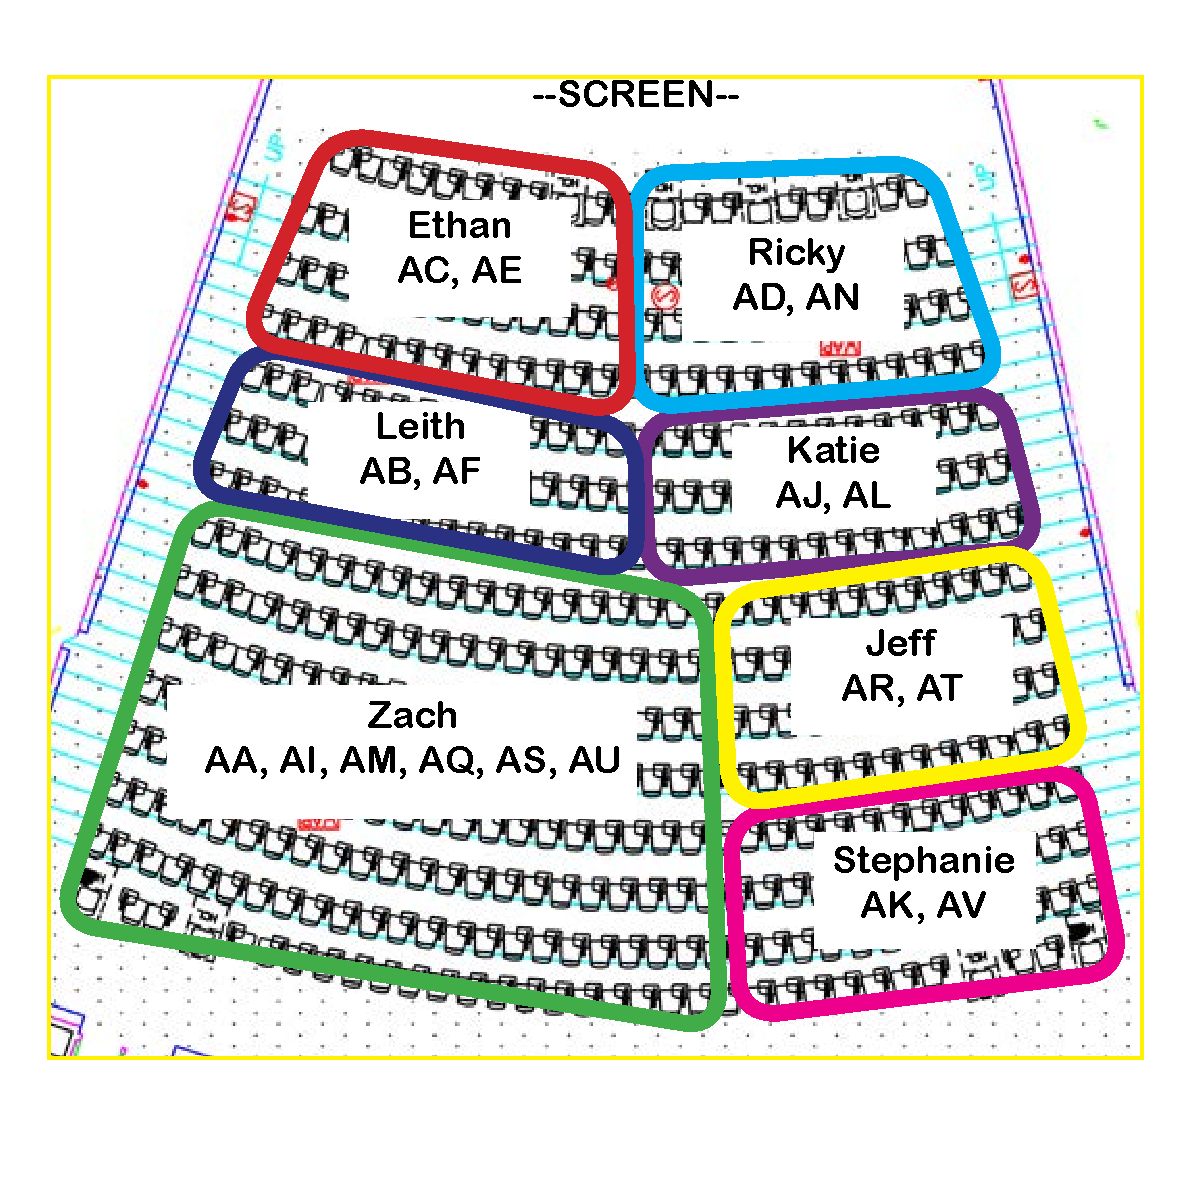
\includegraphics[height=1.2\textheight]{../images/seating-chart.pdf}
    \end{center}
\end{frame}
\end{noheadline}
}

\begin{noheadline}
\begin{frame}
\frametitle{Today's issues:}
\vspace{5mm}
\tableofcontents[subsectionstyle=hide]
\end{frame}
\end{noheadline}

\section{Will blondes go extinct?}



\begin{noheadline}
\begin{frame}[t]
    \frametitle{Blondes `to die out in 200 years'\footnote{BBC World Health, 27 September, 2002}}
    \begin{adjustwidth}{-1.5em}{-1.5em}
        \begin{quote}
            The last natural blondes will die out within 200 years, scientists
            believe.  A study by experts in Germany suggests people with blonde
            hair are an endangered species and will become extinct by 2202.
            Researchers predict the last truly natural blonde will be born in
            Finland---the country with the highest proportion of blondes.  But
            they say too few people now carry the gene for blondes to last
            beyond the next two centuries.

            \vspace{4mm}
            \highlight{The problem is that blonde hair is caused by a recessive
                gene.}  In order for a child to have blonde hair, it must have
            the gene on both sides of the family in the grandparents'
            generation \ldots
        \end{quote}

    \end{adjustwidth}
\end{frame}
\end{noheadline}

\begin{noheadline}
\begin{frame}[t]
    \begin{adjustwidth}{-1.5em}{-1.5em}

        \begin{itemize}
            \item Use the exercise on the worksheet to figure out whether
                blondes are going extinct. Please print your names legibly. 

                \vspace{1cm}
            \item Work in teams of 3---middle person is the scribe (should do the
                writing).  Make sure that you can explain your reasoning in
                each step. 

                \vspace{1cm}
            \item We'll do a series of clicker questions when everyone is done
                with page 1 \ldots but go ahead and start working on page 2 if
                you are faster than most groups. 
        \end{itemize}
    \end{adjustwidth}
\end{frame}
\end{noheadline}

\clickerslide{
\begin{frame}[t]
    \begin{clickerquestion}
        \item Suppose that blondes have higher fitness---meaning that they
            produce more offspring than non-blondes.  Would your answer to Q4
            be the same?
 
        \begin{clickeroptions}
            \item \clickeranswer{No, because the recessive allele for blonde
                    hair would appear more often in the \f{1}s due to higher
                    fitness.}
            \item No, because if blondes have higher fitness, then blondes
                would be dominant and not recessive---therefore proportions
                would switch.
            \item Yes, because the number of offspring does not depend on the
                allele frequency for blondes.
            \item Yes---the frequency of the alleles would be different, but it
                would not result in a change in frequency from one generation
                to the next.
        \end{clickeroptions}
    \end{clickerquestion}
\end{frame}
}

\clickerslide{
\begin{frame}[t]
    \begin{clickerquestion}
        \item Suppose that immigration from Finland suddenly increased
            dramatically and a large number of Finnish citizens joined the
            \f{1}s in the U.S.  Would your answer to Q4 be the same? 
 
        \begin{clickeroptions}
            \item No, because the blonde allele is still recessive and
                therefore ratios would be the same. 
            \item \clickeranswer{No, because the population would have more
                    recessive alleles.}
            \item Yes, because originally the frequency would change, but the
                new frequency would stay constant with subsequent generations.
            \item Yes, because the number of individuals won't change the
                frequency in a population. 
        \end{clickeroptions}
    \end{clickerquestion}
\end{frame}
}

\clickerslide{
\begin{frame}[t]
    \begin{clickerquestion}
        \item Suppose that a mutation in the parental population converted some
            of the $a$ alleles to $a\prime$, a brand new allele.  Would your
            answer to Q4 be the same? 
 
        \begin{clickeroptions}
            \item Yes and no. It depends if $a\prime$ is dominant or recessive.
                If recessive, then the same. If dominant, then different. 
            \item Yes. It would decrease initial frequencies but not subsequent
                frequencies.
            \item \clickeranswer{No, because a new allele $a\prime$ would
                    change the frequencies of the alleles in the population.}
            \item No---mutations add new variations in the population but don't
                change existing frequencies. 
        \end{clickeroptions}
    \end{clickerquestion}
\end{frame}
}

\clickerslide{
\begin{frame}[t]
    \begin{clickerquestion}
        \item Suppose that when gametes from the parental generation were
            combining to form \f{1} offspring, by chance many more $A$ alleles
            ended up in \f{1} offspring than predicted by their actual
            frequency. Would your answer to Q4 be the same?
 
        \begin{clickeroptions}
            \item \clickeranswer{No---the frequency has changed in the \f{1}s,
                    even though it occurred by chance.}
            \item No, because it was just by chance. So later generations would
                balance out.
            \item Yes, because the population has not been changed.
            \item Yes---the randomness of sperm and egg combination is
                independent from this prediction.
        \end{clickeroptions}
    \end{clickerquestion}
\end{frame}
}

\clickerslide{
\begin{frame}[t]
    \begin{clickerquestion}
        \item Suppose that non-blondes preferred to breed with other
            non-blondes, so were less likely to breed with blondes. But blondes
            could still breed with blondes. Would your answer to Q4 be the
            same?
 
        \begin{clickeroptions}
            \item It depends on whether the individuals are heterozygous or
                homozygous, but the frequencies would still be changing. 
            \item No, since the frequency in Q4 was based on random
                outcrossing. 
            \item \clickeranswer{Yes---as long as blondes and non-blondes
                    produce the same number of offspring, allele frequencies
                    will stay the same.}
            \item Yes---the non-blondes would be carriers of a blonde allele, so
                the allele frequency would remain unchanged.
        \end{clickeroptions}
    \end{clickerquestion}
\end{frame}
}

\whiteslide

\begin{noheadline}
\begin{frame}
    \small

    \begin{adjustwidth}{-1.5em}{-1.5em}
    \vspace{-0.3cm}
    \begin{columns}
        \column{0.5\textwidth}
    Problem 1: Survey 100 humans; determine genotypes at the $MN$ blood type
    locus.

        \column{0.5\textwidth}
    \begin{table}%[htbp]
        \small
        \centering
        \begin{tabular}{ p{1cm} p{1cm} p{1cm} }
            \toprule
            $MM$ & {$MN$} & {$NN$} \\
            \hline
            18 & 50 & 32 \\
            \bottomrule
        \end{tabular}
    \end{table}
    \end{columns}

    \vspace{2mm}
    \begin{enumerate}
            \small
        \item What is the observed frequency of the genotypes? 
            \nbox{\tiny $MM$: $18/100 = 0.18$; $MN$: $50/100 = 0.5$; $NN$: $32/100
                = 0.32$}

        \item What is the observed frequency of the $M$ and $N$ alleles?
        \begin{tabular}{ p{4cm} p{1cm} }
            $fr(M) = $ & $fr(N) = $ \\
        \end{tabular}
        \nbox{\tiny $fr(M) = ((18 \times 2) + 50)/200 = 86/200 = 0.43$
                    \hspace{1em}OR\hspace{1em}
                    $fr(M) = 0.18 + (0.5/2) = 0.43$ \\
            $fr(N) = ((32 \times 2) + 50)/200 = 114/200 = 0.57$
            \hspace{1em}OR\hspace{1em}
            $fr(M) = 0.32 + (0.5/2) = 0.57$}
        
        \item Given the observed allele frequencies, what are the expected
            genotype frequencies under the null hypothesis of no evolution and
            random mating with respect to the blood type gene?
            \nbox{\tiny   $fr(MM) = 0.43^2 = 0.185$ \\
                        $fr(MN) = 2(0.43)(0.57) = 0.49$ \\
                        $fr(NN) = 0.57^2$}

        \item Compare the observed and expected values: Do the data support the
            null hypothesis?
            \nbox{\tiny What kind of test should we use? Goodness-of-fit test}
    \end{enumerate}
    \end{adjustwidth}
\end{frame}
\end{noheadline}

\end{document}

\clickerslide{
\begin{frame}
    \begin{clickerquestion}
        \item 
        \begin{clickeroptions}
            \item 
            \item 
            \item 
            \item 
        \end{clickeroptions}
    \end{clickerquestion}
\end{frame}
}
